\chapter{Management Abläufe}

\section{Kostenvoranschlag}
\begin{itemize}
    \item Vier Entwickler während 14 Wochen
    \item Projektstart am 20. Februar 2014
    \item Projektende am 30. Mai 2014
    \item Wöchentlicher Aufwand 10 Stunden/Entwickler
    \item Aufwand Total: 14 Wochen * 10 Stunden * 8 Entwickler = 560 Stunden
\end{itemize}
Werden die Kernfunktionalitäten vorzeitig erfüllt, kann durch den Projektumfang die restliche Zeit vollumfänglich für optionale Funktionalitäten genutzt werden.

\section{Zeitliche Planung}
Wir werden in unserem Projekt nach dem Unified Process arbeiten. Die beinhaltet die Phasen: 
\\\begin{itemize}
    \item Inception
    \item Elaboration
    \item Construction
    \item Transition
\end{itemize}
\begin{figure}[ht]
    \center
    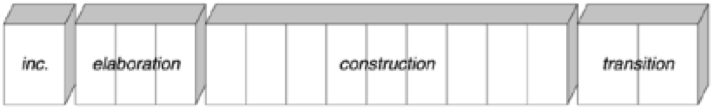
\includegraphics[width=0.8\textwidth]{content/images/unified_process_phasen.png}
    \caption{Unified Process Phasen}
\end{figure}

\section{Iterationsplanung}
\begin{table}[H]
    \tablestyle
    \tablealtcolored
    \begin{tabularx}{\textwidth}{l X p{3.5cm} r}
        \tableheadcolor
            \tablehead Iteration &
            \tablehead Arbeitspaket &
            \tablehead Meilenstein &
            \tablehead SW \tabularnewline
        \tablebody
            \textit{Inception I1} &
            \begin{itemize}
                \item Projektantrag erstellen
                \item Virtueller Server beantragen
                \item Projektplan erstellen
                \item Entwicklungsumgebung einrichten (Client)
                \item Entwicklungsumgebung einrichten (Server)
                \item Vorgabe für Dokumentation erstellen
            \end{itemize} &
            \begin{itemize}
                \item Abgabe Projektantrag
                \item Gemeinsame Vision des Projekts
            \end{itemize} &
            1-2
        \tabularnewline
            \textit{Elaboration E1} &
            \begin{itemize}
                \item Projektplan verfeinern
                \item Domainanalyse
                    \begin{itemize}
                        \item Domainmodell
                        \item System State Diagramm
                        \item Operation Contracts
                    \end{itemize}
                \item Erstellen von Use Cases 
                    \begin{itemize}
                        \item Analyse
                        \item „brief“-Format zu 80%
                        \item „fully dressed“-Format zu 10%
                    \end{itemize}
                \item Erstellung Personas / Szenarios
                \item Anforderungsspezifikation erstellen
                \item Erstellung des Prototyps
                \item Machbarkeitsanalyse erstellen
            \end{itemize} &
            \begin{itemize}
                \item Abgabe MS1-RV. Projektplan
            \end{itemize} &
            2-4
        \tabularnewline
            \textit{Elaboration E2} &
            \begin{itemize}
                \item Entwicklungsumgebung vollständig eingerichtet
                \item Domainanalyse abgeschlossen
                \item Fertigstellung Anforderungsspezifikationen
                \item Fertigstellung Use Cases
                \item Fertigstellung Architektur-Prototyps
            \end{itemize} &
            \begin{itemize}
                \item MS2-RV. Anforderungen und Analyse
            \end{itemize} &
            5-6
        \tabularnewline
            \textit{Construction C1} &
            \begin{itemize}
                \item Implementationsarbeiten beginnen
                    \begin{itemize}
                        \item Login-/Logout-Funktion
                        \item Einsatzkatalog 
                        \item Mitgliederverwaltung
                    \end{itemize}
                \item Anpassungen gemäss Designreview
            \end{itemize} &
            \begin{itemize}
                \item MS3-RV. Ende Elaboration
            \end{itemize} &
            7-8
        \tabularnewline
        \tableend
    \end{tabularx}
    \caption{Iterationsplanung (1/2)}
\end{table}

\begin{table}[H]
    \tablestyle
    \tablealtcolored
    \begin{tabularx}{\textwidth}{l X p{3.5cm} r}
        \tableheadcolor
            \tablehead Iteration &
            \tablehead Arbeitspaket &
            \tablehead Meilenstein &
            \tablehead SW \tabularnewline
        \tablebody
            \textit{Construction C2} &
            \begin{itemize}
                \item Externes Design anpassen
                \item Implementationen erweitern
                    \begin{itemize}
                        \item Unit Testing
                        \item Helfereinsätze importieren
                        \item Einsatzverwaltung
                    \end{itemize}
            \end{itemize} &
            \begin{itemize}
                \item MS4-RV. Architektur/Design
            \end{itemize} &
            9-10
        \tabularnewline
            \textit{Construction C3} &
            \begin{itemize}
                \item Implementationen abschliessen
                    \begin{itemize}
                        \item Import- / Export-Funktionen
                        \item Optionale Funktionalitäten
                    \end{itemize}
                \item Testing 
                \item Reserven für Risiken
            \end{itemize} &
            \begin{itemize}
                \item MS2-RV. Anforderungen und Analyse
            \end{itemize} &
            11-12
        \tabularnewline
            \textit{Transition T1} &
            \begin{itemize}
                \item Präsentation vorbereiten
                \item Abschlussbericht verfassen
            \end{itemize} &
            \begin{itemize}
                \item MS5. Schlusspräsentation/-abgabe
            \end{itemize} &
            13-14
        \tabularnewline
        \tableend
    \end{tabularx}
    \caption{Iterationsplanung (2/2)}
\end{table}

\section{Meilensteine}
\begin{table}[H]
    \tablestyle
    \tablealtcolored
    \begin{tabularx}{\textwidth}{l|l|X|X|r}
    \tableheadcolor
        \tablehead Start & \tablehead Ende & \tablehead Meilenstein & \tablehead Deliverables & \tablehead Phase
        \tabularnewline
    \tablebody
        20.02.14 & 21.02.14 & Projektantrag & Projektantrag & I1 
        \tabularnewline 
         & 07.03.14 & Projektplan & Projektplan & E1 
        \tabularnewline 
         &  & Anforderungen und Analyse &  & E2 
        \tabularnewline 
         &  & Ende Elaboration &  & C1 
        \tabularnewline 
         &  & Architektur und Design &  & C2 
        \tabularnewline 
         &  &  &  & C3 
        \tabularnewline 
         &  & Schlusspräsentation & & T1 
        \tabularnewline 
    \tableend
    \end{tabularx}
    \caption{Meilensteine}
\end{table}

\section{Besprechungen}
Es wird wöchentlich mindestens eine fixe Teamsitzung mit allen Projektbeteiligten durchgeführt. Diese wird jeweils am Donnerstag stattfinden und zwischen ein bis zwei Stunden andauern. 
\\Sie dienen dem Zweck, getätigte Arbeiten mitzuteilen, bevorstehende Arbeiten gemeinsam zu planen und offene Fragen zu beantworten. Falls nötig, können weitere Sitzungen einberufen werden. 

